%!TEX root = da2020-11.tex

\Chapter{11}{Hardness of Coloring}

\noindent
This week we will apply round elimination to coloring. We will show that 3-coloring paths requires $\Omega(\log^* n)$ rounds. This matches the fast coloring algorithms that we saw in Chapter~\chapterref{1}.

To prove this result, we will see how to apply round elimination to randomized algorithms. Previously round elimination was purely deterministic: a $T$-round deterministic algorithm would imply a $(T-1)$-round deterministic algorithm for the output problem. With randomized algorithms, round elimination affects the success probability of the algorithm: a $T$-round randomized algorithm implies a $(T-1)$-round randomized algorithm for the output problem with a worse success probability.

We will see how round elimination can be applied in the presence of inputs. These inputs can be, in addition to randomness, e.g.\ a coloring or an orientation of the edges. The critical property for round elimination is that there are no \emph{long range dependencies} in the input.

\section{Coloring and Round Elimination}

We begin by applying round elimination to coloring on paths, or $(2,2)$-biregular trees. For technical reasons, we also encode a consistent orientation in the coloring. That is, in addition to computing a coloring, we require that the nodes also orient the path consistently from one endpoint to the other. This is a hard problem, as we saw in the previous chapter; therefore we will assume that the input is \emph{already oriented}. We will show that $3$-coloring a path requires $\Omega(\log^* n)$ rounds \emph{even if the path is consistently oriented}.

\subsection{Encoding Coloring}

\begin{figure}
	\centering
	\includegraphics[page=\PEncodingThreeColoring,scale=0.4]{figs.pdf}
	\caption{Encoding of 3-coloring in the bipartite formalism. On top, a 3-coloring of a path fragment. Below, the corresponding 3-coloring as a bipartite locally verifiable problem. The path is assumed to be consistently oriented, so each node has an incoming and an outgoing edge. They use the regular label on the incoming edge, and the barred label on the outgoing edge. Passive nodes verify that the colors differ and have different type.} \label{fig:3col-encoding}
\end{figure}

We will study the problem of $3$-coloring the \emph{active nodes} of a $(2,2)$-biregular tree. We will say that two active nodes are \emph{adjacent} if they share a passive neighbor. 

To encode the orientation, we use two versions of each color label: e.g.\ 1 and $\bar{1}$. We call these \emph{regular} and \emph{barred} labels, respectively. For 3-coloring, we have the following problem $\Pi_0 = (\Sigma_0, \collA_0, \collP_0)$:
\begin{align*}
	\Sigma_0 &= \{ 1,\bar{1},2,\bar{2},3,\bar{3} \}, \\
	\collA_0 &= \bigl\{ [ 1, \bar{1} ],\, [2,\bar{2}],\, [3,\bar{3}] \bigr\}, \\
	\collP_0 &= \bigl\{ [ 1, \bar{2}],\, [1, \bar{3}],\, [2, \bar{1}],\, [2, \bar{3}],\,[3,\bar{1}],\,[3,\bar{2}] \bigr\}.
\end{align*}
The encoding of 3-coloring is shown in Figure~\ref{fig:3col-encoding}. The active configurations ensure that each node chooses a color and an orientation of its edges: we can think of the edges labeled with $\bar{1}$, $\bar{2}$ or $\bar{3}$ as outgoing edges, and the regular labels as incoming edges. The passive configurations ensure that adjacent active nodes are properly colored and that the passive node is properly oriented (has incident labels of different types).

We will also need to define coloring with more colors. We say that a label \emph{matches} with its barred version: $1 \sim \bar{1}$, $2 \sim \bar{2}$ and so on. A label \emph{does not match} with the other labels: e.g.\ $1 \nsim \bar{2}$. 

We define $c$-coloring as the following problem $\Pi = (\Sigma, \collA, \collP)$:
\begin{align*}
	\Sigma &= \{ 1,\bar{1},2,\bar{2},\dots,c,\bar{c} \}, \\
	\collA &= \bigl\{ [ x, \bar x ] \bigm| x \in \{1,2,\dots,c\} \bigr\}, \\
	\collP &= \bigl\{ [ x, \bar y ] \bigm| x, y \in \{1,2,\dots,c\},\, x \nsim \bar y \bigr\}.
\end{align*}

\subsection{Output Problem of Coloring}

We start by assuming that we have a fast algorithm that solves the $3$-coloring problem $\Pi_0$. Let us now compute the output problem $\Pi_1 = \re(\Pi_0)$ of $3$-coloring~$\Pi_0$.

Let $\Pi_1 = (\Sigma_1, \collA_1, \collP_1)$ denote the output problem. For now, we will let $\Sigma_1$ consist of all non-empty subsets of $\Sigma_0$, and prune it later.

Recall that passive configurations $\collP_0$ consist of all non-matching pairs of a regular and barred label. Therefore the active configurations in $\Pi_1$ consist of all pairs of sets such that
\begin{itemize}[noitemsep]
	\item one set consists of regular and one of barred labels, and
	\item there are no matching labels.
\end{itemize}
We get that
\[
	\collA_1 = \bigl\{ [X,Y] \bigm| X \subseteq \{1,2,3\}, Y \subseteq \{\bar{1},\bar{2},\bar{3}\}, \forall x \in X, y \in Y: x \nsim y \bigr\}.
\]

Next we make the sets maximal: when neither the regular or the barred version of a label is contained in either set, we can add the corresponding variant to either set. Thus the maximal active configurations \emph{split} the color set over their edges:
\[\begin{split}
	\collA_1 = \Bigl\{& 
	\bigl[\{1\},\{\bar{2},\bar{3}\}\bigr],\,
	\bigl[\{2\},\{\bar{1},\bar{3}\}\bigr],\,
	\bigl[\{3\},\{\bar{1},\bar{2}\}\bigr],\, \\
	&\bigl[\{\bar{1}\},\{2,3\}\bigr],\,
	\bigl[\{\bar{2}\},\{1,3\}\bigr],\,
	\bigl[\{\bar{3}\},\{1,2\}\bigr] 
	\Bigr\}
\end{split}\]
No label can be added to any of the configurations, and the above labels contain all active configurations.

We have the following alphabet: 
\[\begin{split}
	\Sigma_1 = \bigl\{& 
	\{1\}, \{2\}, \{3\}, \{1,2\},\{1,3\}, \{2,3\}, \\
	&\{\bar{1}\}, \{\bar{2}\}, \{\bar{3}\}, \{\bar{1},\bar{2}\},\{\bar{1},\bar{3}\}, \{\bar{2},\bar{3}\} \bigr\}.
\end{split}\]

Finally, the passive configurations consist of all pairs such that it is possible to pick matching regular and barred labels, forming a configuration in $\collA_0$:
\[
	\collP_1 = \bigl\{ [X,Y] \bigm| (1 \in X, \bar{1} \in Y) \vee (2 \in X, \bar{2} \in Y) \vee (3 \in X, \bar{3} \in Y) \bigr\}.
\]

\subsection{Simplification}

The output problem of 3-coloring looks much more complicated than the problem we started with. If we kept applying round elimination, it would become extremely difficult to understand the structure of the problem. Therefore we will \emph{simplify} the problem: we will map it back to a coloring with a \emph{larger number of colors}.

The intuition is the following. Assume that our original labels consist of some set of $c$ colors, and the output problem has sets of these colors as labels. Then there are at most $2^c$ different sets. If adjacent nodes have always different sets, we can treat it as a coloring with $2^c$ colors by mapping the sets to the labels $1,2,\dots, 2^c$.

Now consider the output problem of 3-coloring, $\Pi_1$. We will treat the different sets of the regular labels as the color classes. Each of them is paired with a unique set of barred labels. Enumerating all options, we rename the labels as follows to match the alphabet of $6$-coloring:
\begingroup
\allowdisplaybreaks
\begin{alignat*}{2}
	\{ 1 \} &\mapsto 1, & \quad\{\bar{2},\bar{3} \} &\mapsto \bar{1}, \\
	\{ 2 \} &\mapsto 2, & \{\bar{1},\bar{3} \} &\mapsto \bar{2}, \\
	\{ 3 \} &\mapsto 3, & \{\bar{1},\bar{2} \} &\mapsto \bar{3}, \\
	\{ 1,2 \} &\mapsto 4, & \{\bar{3}\} &\mapsto \bar{4}, \\
	\{ 1,3 \} &\mapsto 5, & \{ \bar{2} \} &\mapsto \bar{5}, \\
	\{ 2,3 \} &\mapsto 6, & \{ \bar{1} \} &\mapsto \bar{6}.
\end{alignat*}
\endgroup

Now let us verify that this is indeed a 6-coloring. After renaming, the active configurations are
\begin{align*}
	\collA_1 = \bigl\{& 
	[1,\bar{1}],\,
	[2,\bar{2}],\,
	[3,\bar{3}],\, \\
	&[\bar{6},6],\,
	[\bar{5},5],\,
	[\bar{4},4] 
	\bigr\}.
\end{align*}
By rearrangement we can see that these match exactly the definition of $6$-coloring. The passive configurations, before renaming, were the pairs of sets, one consisting of the regular labels and the other of the barred labels, that contained a matching label. We get that 
\begin{align*}
	\collP_1
	      = {}&\bigl\{ [1, x] \bigm| x \in \{ \bar{2}, \bar{3}, \bar{6} \} \bigr\} \\
	{} \cup {}&\bigl\{ [2, x] \bigm| x \in \{ \bar{1}, \bar{3}, \bar{5} \} \bigr\} \\
	{} \cup {}&\bigl\{ [3, x] \bigm| x \in \{ \bar{1}, \bar{2}, \bar{4} \} \bigr\} \\
	{} \cup {}&\bigl\{ [4, x] \bigm| x \in \{ \bar{1}, \bar{2}, \bar{3}, \bar{5}, \bar{6} \} \bigr\} \\
	{} \cup {}&\bigl\{ [5, x] \bigm| x \in \{ \bar{1}, \bar{2}, \bar{3}, \bar{4}, \bar{6} \} \bigr\} \\
	{} \cup {}&\bigl\{ [6, x] \bigm| x \in \{ \bar{1}, \bar{2}, \bar{3}, \bar{4}, \bar{5} \} \bigr\}.
\end{align*}

We notice that these are a subset of the passive configurations of 6-coloring: colors 1, 2, and 3 cannot be paired with some of the non-matching colors. This means that $\Pi_1$ is \emph{at least as hard} to solve as 6-coloring.

We may \emph{relax} the output problem $\Pi_1$ and construct a new problem $\Pi'_1 = (\Sigma'_1, \collA'_1, \collP'_1)$ as follows:
\begingroup
\allowdisplaybreaks
\begin{align*}
 \collA'_1 = {}&\collA_1,\\
 \collP'_1
       = {}&\bigl\{ [1, x] \bigm| x \in \{ \bar{2}, \bar{3}, \bar{4}, \bar{5}, \bar{6} \} \bigr\} \\
 {} \cup {}&\bigl\{ [2, x] \bigm| x \in \{ \bar{1}, \bar{3}, \bar{4}, \bar{5}, \bar{6} \} \bigr\} \\
 {} \cup {}&\bigl\{ [3, x] \bigm| x \in \{ \bar{1}, \bar{2}, \bar{4}, \bar{5}, \bar{6} \} \bigr\} \\
 {} \cup {}&\bigl\{ [4, x] \bigm| x \in \{ \bar{1}, \bar{2}, \bar{3}, \bar{5}, \bar{6} \} \bigr\} \\
 {} \cup {}&\bigl\{ [5, x] \bigm| x \in \{ \bar{1}, \bar{2}, \bar{3}, \bar{4}, \bar{6} \} \bigr\} \\
 {} \cup {}&\bigl\{ [6, x] \bigm| x \in \{ \bar{1}, \bar{2}, \bar{3}, \bar{4}, \bar{5} \} \bigr\}.
\end{align*}
\endgroup
Note that $\Pi'_1$ is exactly the $6$-coloring problem. As we have got that $\collA'_1 = \collA_1$ and $\collP'_1 \supseteq \collP_1$, any solution to $\Pi_1$ is also a solution to $\Pi'_1$. We conclude that if we can solve problem $\Pi_0$ in $T$ rounds, we can solve $\Pi_1 = \re(\Pi_0)$ \emph{exactly} one round faster, and we can solve its relaxation $\Pi'_1$ \emph{at least} one round faster.

\subsection{Generalizing Round Elimination for Coloring}

Let us now see how to generalize the first round elimination step. In the first step, we saw that 6-coloring is at least as easy to solve as the output problem of 3-coloring.

Now consider applying round elimination to the $c$-coloring problem. Let $\re(\Pi_0) = \Pi_1 = (\Sigma_1,\collA_1, \collP_1)$ denote the output problem of $c$-coloring $\Pi_0$.

Again, the active configurations in $\collA_1$ consist of all splits of the colors. For a set $X \subseteq \{1,2,\dots,c\}$, let $\bar{X}$ denote the \emph{barred complement of $X$}:
\[
	\bar{X} = \{ \bar{x} \bigm| x \in \{ 1,2,\dots,c\} \setminus X \}.
\]
Then the active configurations are 
\[
	\collA_1 = \bigl\{ [X, \bar{X}] \bigm| \emptyset \ne X \subsetneq \{1,2,\dots,c\} \bigr\}.
\]
The labels are all non-empty and non-full subsets of the regular and barred labels, respectively. The passive configurations in $\collP_1$ consists of pairs of sets such that it is possible to pick matching regular and barred labels from them:
\[
	\collP_1 = \bigl\{ [X,Y] \bigm| x \in X, \bar{x} \in Y: x \sim \bar{x} \bigr\}.
\]
We do the exact same renaming trick as in the previous section. There are a total of $2^c - 2$ different sets on regular labels. We rename them in some order with the integers from $1$ to $2^c-2$. For each set $X$ renamed to integer $y$, we rename the unique barred complement $\bar{X}$ to $\bar{y}$. The active configurations after renaming are
\[
	\collA_1 = \bigl\{ [x,\bar{x}] \bigm| x \in \{1,2,\dots, 2^c-2 \} \bigr\}.
\]
We note that passive configurations never include $[x,\bar{x}]$ for any $x$. This is because $\bar{x}$ represents the complement of $x$ as a set: it is not possible to pick a matching element from $x$ and $\bar{x}$. Therefore we may again \emph{relax} the passive configurations to be the configurations for $c$-coloring:
\[
	\collP_1 = \bigl\{ [x,\bar y] \bigm| x, y \in \{1,2,\dots,2^c-2\},\, x \nsim \bar y \bigr\}.
\]
The resulting problem is \emph{at least as easy} as the output problem of $c$-coloring: if $c$-coloring can be solved in $T$ rounds, then coloring with $2^c-2$ colors can be solved in \emph{at most} $T-1$ rounds.

Now in what follows, it will be awkward to use the expression $2^c-2$, so we will simply round it up to $2^c$. Clearly, coloring with $2^c$ colors is at least as easy as coloring with $2^c-2$ colors.

\subsection{Sequence of Output Problems}

We have shown that $2^c$-coloring is \emph{at least as easy} as the output problem of $c$-coloring. 
Now if we were to iteratively apply round elimination $k$ times in the $\PN$-model we would get the following sequence of problems:
\[\begin{split}
	\Pi_0 = 3\text{-coloring}
	&\to \Pi_1 = 2^3\text{-coloring} \\
	&\to \Pi_2 = 2^{2^3}\text{-coloring} \\
	&\to \Pi_3 = 2^{2^{2^3}}\text{-coloring} \\
	&\phantom{{}\to{}} {\cdots} \\
	&\to \Pi_k = C(k)\text{-coloring},
\end{split}\]
where
\[
	C(k) = \underbrace{\,2^{2^{\scriptstyle\cdot^{\scriptstyle\cdot^{\scriptstyle\cdot^{\scriptstyle 2^{\scriptstyle 3}}}}}}}_{\text{\makebox[0pt]{$k$ times $2$ and one $3$}}}.
\]
Now if we show that coloring with $C(k)$ colors cannot be solved in $0$ rounds in the $\PN$ model with deterministic algorithms, it would imply that $3$-coloring cannot be solved in $k$ rounds in the $\PN$ model. This result, however, would not be very meaningful. As we have already seen in Chapter~\chapterref{7}, the vertex coloring problem cannot be solved at all in the $\PN$-model! Therefore we must strengthen the round elimination technique itself to apply in the $\LOCAL$ model.

\section{Round Elimination with Inputs}

If we try to do round elimination in the $\LOCAL$ model, we run into a technical challenge. In round elimination, the nodes simulate the outputs of their neighbors. It is crucial that the inputs of the neighbors are independent: for each combination of possible outputs, there must exist a network in which the algorithm actually produces those outputs. This step no longer holds in the $\LOCAL$ model: the identifiers are globally unique, and therefore do not repeat. The inputs of the neighbors \emph{are dependent}: if one of the regions contains, e.g., a node with identifier 1, then another region cannot contain identifier 1, and vice versa.

To overcome this difficulty, we will consider \emph{randomized algorithms}. In Exercise~\longref{6.2}{ex:randomness-to-unique-ids} we saw that randomness can be used to generate unique identifiers. Therefore the $\PN$-model, equipped with randomness, is at least as powerful as the $\LOCAL$ model: if a problem $\Pi$ can be solved in time $T(n)$ in the $\LOCAL$ model, then we can generate unique identifiers with high probability and simulate the $\LOCAL$-algorithm in $T(n)$ rounds. This clearly succeeds if the random identifiers were unique. Therefore any impossibility results we prove for randomized algorithms also hold for the $\LOCAL$ model.

For the remainder of the chapter, we assume that the nodes receive two types of inputs.
\begin{enumerate}
	\item Random inputs. Each node receives some arbitrary but finite number of uniform random bits as input. In addition, to simplify the proof, we will assume that the port numbers are assigned randomly. This latter assumption is made only for the purposes of this proof, we do not change the standard assumptions about the models.
	\item Consistent orientation. As we mentioned in the beginning, for technical reasons we consider a variant of coloring that includes an orientation. To solve this part of the problem easily, we include the required orientation as input.
\end{enumerate}
It is crucial that we can apply round elimination in the presence of these inputs. First, consider the orientation. In the round elimination step, each node must simulate the outputs of its neighbors over all possible inputs. Now we add the promise that each node, in addition to its usual inputs, receives an orientation of its edges as input. In particular, they forms a \emph{consistent orientation} of the whole path from one end to the other. Clearly nodes can include this input in their simulation, as the orientation of the remaining edges is fixed after seeing the orientation of just one edge. Similarly, random inputs do not have any long-range dependencies. They do, however, affect the simulation step. We will discuss randomized round elimination in the next section.

\subsection{Randomized Round Elimination Step} \label{ssec:rand-re}

We will now introduce a variant of the Round Elimination Lemma that we proved in Chapter~\chapterref{9}. Assume that we have a randomized algorithm that solves problem $\Pi$ in $T(n)$ rounds with \emph{local failure probability $q$}: that is, each active node chooses an active configuration of $\Pi$ with probability \emph{at least} $1-q$, and each passive node is labeled according to some passive configuration of $\Pi$ with probability \emph{at least} $1-q$. Then we want to show that there is an algorithm that solves the output problem $\re(\Pi)$ in $T(n)-1$ rounds with some local failure probability at most $f(q)$ for some function $f$.

\begin{figure}
	\centering
	\includegraphics[page=\PRandomizedRE,scale=0.4]{figs.pdf}
	\caption{The randomized round elimination step. Assume an algorithm $A$ for $c$-coloring with running time $T = 3$. The simulation functions as follows. The active node gathers its $(T-1)$-neighborhood, including the assignment of random port numbers and random bits $r_1, r_2, r_3, r_4$ and $r_5$. Then it simulates $A$ on its right and left neighbor. On the right, over all possible assignments of ports $A, B, C$, $D$ and random bit strings $X, Y$. On the left, over all possible assignments of ports $E,F,G,H$ and random bit strings $Z,W$. For each edge, it outputs the set of labels that appear as outputs for at least fraction $t(q)$ of inputs.} \label{fig:rand-re}
\end{figure}

The round elimination step works essentially as in the $\PN$-model. Each $\re(\Pi)$-active node simulates the outputs of its $\Pi$-active nodes over all possible inputs, including the random bits. We make one modification to the model: we assume that the port numbers are assigned randomly instead of being assigned by an adversary. This modification is made to simplify the analysis that follows. It does not affect the power of the model: the nodes could use their local randomness to shuffle the ports and any algorithm designed for the worst-case port numbering also works, by definition, with a random port numbering. We will also only consider nodes that are internal nodes in the $(2,2)$-biregular tree: we assume that $T$-neighborhoods of the neighbors of $\re(\Pi)$-active nodes do not contain the endpoints of the path.

It no longer makes sense to construct the set of \emph{all possible} outputs. We can imagine an algorithm that tries to make round elimination hard: it always uses each possible output label with at least one specific random input labeling. These outputs would make no sense, but would cause the set of \emph{possible} output labels to always be the full set of labels. Since the random inputs can be arbitrarily large (but finite!), the failure probability this would add to the algorithm would be small.

To avoid this issue, we will define a \emph{threshold $t(q)$}: an output label $\sigma \in \Sigma$ is \emph{frequent} if it appears as the output label with probability at least $t(q)$. 
More formally, for a fixed $\re(\Pi)$-active node $u$, an assignment of random inputs to $\ball_N(u,T-1)$, and a neighbor $v$, label $\sigma \in \Sigma$ is frequent for the edge $\{ u, v \}$ if the probability that $v$ outputs $\sigma$ on $\{u,v\}$, conditioned on fixing the random inputs in $\ball_N(u, T-1)$, is at least $t(q)$. We will fix the value of this threshold later.

The randomized simulation step is defined as follows. Each $\Pi_1$-active node $u$ gathers its $(T-1)$-neighborhood. Then it computes for each edge $\{u,v\}$ the set of frequent labels $S(u,v)$ and outputs that set on $\{u,v\}$. See Figure~\ref{fig:rand-re} for an illustration.

We will prove that randomized round elimination works for the special case of $c$-coloring $(2,2)$-biregular trees. This can be generalized to cover all bipartite locally verifiable problems in $(d,\delta)$-biregular trees, for any parameters $d$ and $\delta$.

\begin{lemma}[Randomized Round Elimination Lemma] \label{lem:rand-re}
	Assume that there is an algorithm that solves the $c$-coloring problem on $(2,2)$-biregular trees in the randomized $\PN$-model in $T(n)$ rounds with local failure probability at most $q$. Then there exists an algorithm that solves the $2^c$-coloring problem in $T(n)-1$ rounds with local failure probability at most $3cq^{1/3}$.
\end{lemma}

Intuitively the lemma is true, as in most neighborhoods the true outputs must also appear frequently in the simulation. Similarly, combinations of non-configurations cannot be frequent too often, as this would imply that the original algorithms also fails often.

We prove the lemma in Section~\ref{ssec:rand-re-proof}. Next we will see how to apply it to prove an impossibility result for 3-coloring.

\section{Iterated Randomized Round Elimination}

Given the randomized round elimination lemma, we will proceed as follows.
\begin{enumerate}[label=(\arabic*)]
	\item Assume there is a randomized $(\log^* n - 4)$-round algorithm for solving 3-coloring on \emph{consistently oriented} $(2,2)$-biregular trees. Since randomized algorithms are assumed to succeed \emph{with high probability}, the local failure probability $q_0$ must be at most $1/n^k$ for some constant $k$.
	\item Apply randomized round elimination $T(n) = \log^* n - 4$ times to get a $0$-round randomized algorithm for $c_{T(n)}$-coloring with some local failure probability $q_{T(n)}$. For the chosen value of $T(n)$ show that we have $q_{T(n)} < 1/c_{T(n)}$. \label{item:part2}
	\item Prove that there are no 0-round algorithms for solving $c_{T(n)}$-coloring with local failure probability $q_{T(n)} < 1/c_{T(n)}$. \label{item:part3} 
\end{enumerate}

We must show that fast coloring algorithms imply 0-round coloring algorithms that do not fail with large enough probability. In Section~\ref{ssec:prob-re} we will prove the following lemma.

\begin{lemma} \label{lem:color-re}
	Assume that there is a $(\log^* n - 4)$-round 3-coloring algorithm in the randomized $\PN$-model. Then there is a 0-round $c$-coloring algorithm with local failure probability $q < 1/c$.
\end{lemma}

We must also show that any 0-round $c$-coloring algorithm fails locally with probability at least $1/c$.

\begin{lemma} \label{lem:0round-ccol}
	Any 0-round $c$-coloring algorithm fails locally with probability at least $1/c$.
\end{lemma}

\begin{proof}
	Any 0-round $c$-coloring algorithm defines a probability distribution over the possible output colors. This distribution is the same for each active node inside a path: they are indistinguishable from each other in 0 rounds. The algorithm fails if two adjacent nodes select the same color. 
	
	Let $p_i = b_i + 1/c$ denote the probability that the algorithm outputs color $i$. The terms $b_i$ denote the deviation of each probability $p_i$ from the average: we must have that
	\[
		\sum_{i=1}^c b_i = 0.
	\] 
	The local failure probability is at least
	\begin{align*}
		\sum_{i=1}^c p_i^2 &= \sum_{i=1}^c (b_i + 1/c)^2 \\
		&= \sum_{i=1}^c \bigl(b_i^2 + 2b_i/c + 1/c^2\bigr) \\
		&= 1/c + \biggl(\sum_{i=1}^c b_i^2\biggr) + 2/c \cdot \biggl(\sum_{i=1}^c b_i\biggr) \\
		&= 1/c + \biggl(\sum_{i=1}^c b_i^2\biggr) + 0.
	\end{align*}
	This is clearly minimized by setting $b_i = 0$ for all $i$. Thus the local failure probability is minimized when $p_i = 1/c$ for all $i$, and we get that it is at least $1/c$.
\end{proof}

The bound on the failure probability of 0-round coloring algorithms combined with Lemma~\ref{lem:color-re} shows that there is no 3-coloring algorithm that runs in at most $\log^* n - 4$ rounds in the randomized $\PN$-model, even if we know $n$ and the path is consistently oriented. Since the randomized $\PN$-model can simulate the $\LOCAL$ model with high probability, this implies that there is no (randomized) 3-coloring algorithm in the $\LOCAL$ model that runs in at most $\log^* n - 4$ rounds.

\begin{theorem}
	3-coloring (in the bipartite formalism) cannot be solved in the $\LOCAL$ model in less than $\log^* n - 4$ rounds.
\end{theorem}

\begin{corollary}
	3-coloring (in the usual sense) cannot be solved in the $\LOCAL$ model in less than $\frac{1}{2} \log^* n - 2$ rounds.
\end{corollary}
\begin{proof}
	Distances between nodes increase by a factor of $2$ when we switch to the bipartite encoding (see Figure~\ref{fig:3col-encoding}).
\end{proof}

This result is asymptotically optimal: already in Chapter~\chapterref{1} we saw that paths \emph{can be colored} with 3 colors in time $O(\log^* n)$.

In the final two sections we give the proofs for Lemmas~\ref{lem:rand-re}~and~\ref{lem:color-re}.

\subsection{Proof of Lemma~\ref{lem:rand-re}} \label{ssec:rand-re-proof}

In this section we prove Lemma~\ref{lem:rand-re}. The proof consists of bounding the local failure probability of the simulation algorithm given in Section~\ref{ssec:rand-re}.

\begin{proof}[Proof of Lemma~\ref{lem:rand-re}]
Let $\Pi_0 = (\Sigma_0, \collA_0, \collP_0)$ denote the $c$-coloring problem for some $c$, and let $\Pi_1 = \re(\Pi_0) = (\Sigma_1, \collA_1, \collP_1)$ denote the output problem of $c$-coloring. Assume that there is a $T$-round randomized algorithm $A$ for solving $\Pi_0$ with local failure probability $q$. 
Consider an arbitrary $\Pi_1$-active node $u$ with some fixed $(T-1)$-neighborhood $\ball_N(u,T-1)$ (including the random inputs).

The passive configurations $\collP_0$ consist of pairs $[x, \bar{y}]$ that do not match. The algorithm $A$ fails if it outputs any $x$ and $\bar{x}$, or two labels of the same type on the incident edges of a $\Pi_0$-passive node. We say that the $(T-1)$-neighborhood $\ball_N(u,T-1)$ is \emph{lucky}, if the algorithm $A$ fails in labeling the incident edges of $u$, given $\ball_N(u,T-1)$, with probability less than $t^2$. Here $t$ is the probability threshold for frequent labels; we will choose the value of $t$ later.

We want to prove that most random bit assignments must be lucky, and that in lucky neighborhoods the simulation succeeds with a good probability. We will ignore the other cases, and simply assume that in those cases the simulation can fail.

Consider any fixed $\ball_N(u,T+1)$ \emph{without} the random bits and the random port numbering: since we consider nodes inside the path, the remaining structure is the same for all nodes. The randomness determines whether $A$ succeeds around $u$. Let $L$ denote the event that $\ball_N(u,T-1)$ is lucky. Since we know that $A$ fails in any neighborhood with probability at most $q$, we can bound the probability of a neighborhood \emph{not being lucky} as follows:
\begin{align*}
	\Pr[A \text{ fails at } u] &\geq  
	\Pr[A \text{ fails at } u \mid \text{not } L]\cdot\Pr[\text{not } L] \\
	\implies \Pr[\text{not } L] &\leq \frac{\Pr[A \text{ fails at } u]}{\Pr[A \text{ fails at } u \mid \text{not } L]}
	< \frac{q}{t^2}.
\end{align*}

From now on we will assume that $\ball_N(u,T-1)$ is lucky. Let $v$ and $w$ denote the passive neighbors of $\re(\Pi)$-active node $u$. The simulation fails if and only if the sets $S(u,v)$ and $S(u,w)$ contain labels $x$ and $y$ such that $[x,y] \notin \collP_0$ (all choices do not yield a configuration in $\collP_0$). Since both of these labels are frequent (included in the output), each of them must appear with probability at least $t$ given $\ball_N(u,T-1)$. But since these labels are frequent, we have that the original algorithm fails, given $\ball_N(u,T-1)$ with probability at least $t^2$, and the neighborhood cannot be lucky. We can deduce that the simulation \emph{always succeeds in lucky neighborhoods}. Therefore we have that
\[
	\Pr[\text{simulation fails}] \leq \Pr[\text{not } L] < \frac{q}{t^2}.
\]

Next we must determine the failure probability of the simulation around \emph{passive nodes}. The $\re(\Pi)$-passive nodes succeed when the \emph{true output} of the algorithm is contained in the sets of frequent outputs. For a $\re(\Pi)$-passive neighbor $v$, consider the event that its output on edge $\{u,v\}$ in the original algorithm is not contained in the set of frequent outputs $S(u,v)$ based on $\ball_N(u,T-1)$. By definition, for each fixed $\ball_N(u,T-1)$ each infrequent label is the true output with probability at most $t$. There are $c$ colors, so by union bound one of these is the true output color with probability at most $ct$. There are two neighbors, so by another union bound the total failure probability for a passive node is at most $2ct$. Since the simulation can also fail when the original algorithm fails, we get for each passive node that
\[
	\Pr[\text{simulation fails}] \leq q + 2ct.
\]
To minimize the maximum of the two failure probabilities, we can for example set $t = q^{1/3}$ and get that
\[
	\frac{q}{t^2} = q^{1/3} \leq q + 2cq^{1/3} \leq 3cq^{1/3}. \qedhere
\]
\end{proof}

\subsection{Proof of Lemma~\ref{lem:color-re}} \label{ssec:prob-re}

It remains to show that a fast 3-coloring algorithm implies a 0-round $c$-coloring algorithm that fails locally with a probability less than $1/c$.

\begin{proof}[Proof of Lemma~\ref{lem:color-re}]
Assume there is a $T$-round 3-coloring algorithm that succeeds with high probability. This implies that it has a local failure probability $q_0 \leq 1/n^k$ for some constant $k \ge 1$. Applying the round elimination lemma, this implies the following coloring algorithms and local failure probabilities $q_i$:
\begin{align*}
	C(0) &= 3 \text{ colors: }&& q_0 \leq 1/n^k \leq 1/n, \\
	C(1) &= 2^3 \text{ colors: }&& q_1 \leq 3 C(0) \cdot q_0^{1/3}, \\
	C(2) &= 2^{2^3} \text{ colors: }&& q_2 \leq 3 C(1) \cdot q_1^{1/3} = 3 C(1) \cdot \bigl(3 C(0) \cdot q_0^{1/3}\bigr)^{1/3}.
\end{align*}
Generalizing, we see that after $T$ iterations, the local failure probability is bounded by
\[
	q_T \leq \Biggl( \prod_{i=0}^T 3^{1/3^i} \Biggr)\Biggl( \prod_{i=0}^T C(T-i)^{1/3^i} \Biggr) \cdot n^{-1/3^T},
\]
and the algorithm uses
\[
	C(T) \,=\, 
	\underbrace{\,2^{2^{\scriptstyle\cdot^{\scriptstyle\cdot^{\scriptstyle\cdot^{\scriptstyle 2^{\scriptstyle 3}}}}}}}_{\text{\makebox[0pt]{\parbox{3cm}{\centering $T$ times $2$\\[-5pt]and one $3$}}}}
	\,<\,
	\underbrace{\,2^{2^{\scriptstyle\cdot^{\scriptstyle\cdot^{\scriptstyle\cdot^{\scriptstyle 2^{\scriptstyle 2^{\scriptstyle 2}}}}}}}}_{\text{\makebox[0pt]{$T+2$ times $2$}}}
	\,=\, {}^{T+2} 2
\]
colors. To finish the proof, we must show that for any $T(n) \leq \log^* n - 4$ and for a sufficiently large $n$ we have that $q_T < 1/C(T)$, or, equivalently, $q_T \cdot C(T) < 1$ or
\begin{equation} \label{eq:prob}
	\log q_T + \log C(T) < 0;
\end{equation}
here all logarithms are to the base $2$.
Evaluating the expression $\log q_T$, we get that
\begin{align*}
	\log q_T &\leq \sum_{i=0}^T \frac{1}{3^i} \log 3 + \sum_{i=0}^T \frac{1}{3^i} \log C(T-i) - 3^{-T} \log n \\
	&\leq \frac{3}{2}\log 3 + \frac{3}{2}\log C(T) - 3^{-T} \log n,
\end{align*}
since the sums are converging geometric sums. Therefore
\begin{equation}\label{eq:logqTlogCT}
	\log q_T + \log C(T) \le \frac{3}{2}\log 3 + \frac{5}{2}\log C(T) - 3^{-T} \log n.
\end{equation}
Note that
\[
	n \le {}^{\log^* n} 2 < 2^n.
\]
Therefore for $T = \log^* n - 4$ we have that
\begin{equation}\label{eq:logCT}
	\log C(T) < \log {}^{T+2} 2 = \log \log \log {}^{T+4} 2 < \log \log n.
\end{equation}
On the other hand, for a large enough $n$ we have that
\[
	3^T < 3^{\log^* n} < 3^{\log_3 \log \log n} < \log \log n,
\]
and therefore
\begin{equation}\label{eq:fact3Tlogn}
	3^{-T} \log n > \frac{\log n}{\log \log n}.
\end{equation}
Now \eqref{eq:logCT} and \eqref{eq:fact3Tlogn} imply that for a sufficiently large $n$, term $3^{-T} \log n$ will dominate the right hand side of \eqref{eq:logqTlogCT}, and we will eventually have
\[
	\log q_T + \log C(T) < 0,
\]
which is exactly what we needed for Equation~\eqref{eq:prob}.
\end{proof}

\section{Quiz}
	
Construct the \emph{smallest possible} (i.e., fewest nodes) properly 4-colored cycle $C$ such that the following holds: if you take \emph{any} deterministic 0-round $\PN$-algorithm $A$ and apply it to $C$, then the output of $A$ is not a valid 3-coloring of $C$.

Please note that here we are working in the usual $\PN$ model, exactly as it was originally specified in Chapter~3, and we are doing graph coloring in the usual sense (we do not use the bipartite formalism here).
Please give the answer by listing the $n$ colors of the $n$-cycle $C$.

\section{Exercises}

\begin{ex}[randomized 2-coloring]
	Prove that solving 2-coloring paths in the randomized $\PN$-model requires $\Omega(n)$ rounds.
\end{ex}

\begin{ex}[coloring grids]
	Prove that 5-coloring 2-dimensional grids in the deterministic $\LOCAL$ model requires $\Omega(\log^* n)$ rounds.
	
	A 2-dimensional grid $G = (V,E)$ consists of $n^2$ nodes $v_{i,j}$ for $i,j \in \{1,\dots, n\}$ such that if $i < n$,  add $\{ v_{i,j}, v_{i+1,j} \}$ to $E$ for each $j$, and if $j < n$ add $\{v_{i,j},v_{i,j+1}\}$ to $E$ for each $i$.
	\hint{Show that a fast 5-coloring algorithm could be simulated on any path to 5-color it. Then turn a 5-coloring into a 3-coloring yielding an algorithm that contradicts the 3-coloring lower bound.} 
\end{ex}

\begin{ex}[more colors]
	Prove that cycles cannot be colored with $O(\log^* n)$ colors in $o(\log^* n)$ rounds in the deterministic $\LOCAL$ model.
	\hint{Show that an $O(\log^* n)$-coloring could be used to color cycles fast, which contradicts the lower bound for 3-coloring. Note that our lower bound is for paths: why does it also apply to cycles?}
\end{ex}

\begin{ex}[lying about $n$]
	Show that if a bipartite locally verifiable labeling problem can be solved in $o(\log n)$ rounds in the deterministic $\PN$-model in $(d,\delta)$-biregular trees, then it can be solved in $O(1)$ rounds.
	\hint{Show that we can run an algorithm for graphs of size $n_0$, for some constant $n_0$, on all networks of size $n \geq n_0$, and get a correct solution. In particular, show that for any $T(n) = o(\log n)$ and a sufficiently large $n_0$, networks on $n_0$ nodes are locally indistinguishable from networks on $n$ nodes, for $n \geq n_0$, in $O(T(n))$ rounds.}
\end{ex}

\begin{ex}[hardness of sinkless orientation]
	Let $\Pi$ denote the sinkless orientation problem as defined in Chapter~\chapterref{10}.
	Prove the following.
	\begin{subex}
		\item Sinkless orientation requires $\Omega(\log \log n)$ rounds in the randomized $\PN$-model. \label{hint:so-a}
		\item Sinkless orientation requires $\Omega(\log \log n)$ rounds in the deterministic and randomized $\LOCAL$ model. \label{hint:so-b}
	\end{subex}
	\hint{\ref{hint:so-a} Show that if $\re(\Pi)$ can be solved by a randomized $\PN$-algorithm in $T$ rounds with local failure probability $q$, then it can be solved in $T-1$ rounds with local failure probability $\poly(q)$. Analyze the failure probability over $T$ iterations for $T = o(\log \log n)$ and show that it is $\omega(1)$.}
\end{ex}

\begin{exs}
	Show that sinkless orientation requires $\Omega(\log n)$ rounds in the deterministic $\LOCAL$ model.
	\hint{One approach is the following. Prove that any \emph{deterministic} $o(\log n)$-time algorithm for sinkless orientation implies an $O(\log^* n)$-time deterministic algorithm for sinkless orientation. To prove this speedup, ``lie'' to the algorithm about the size of the graph. Take an algorithm $A$ for $(3,3)$-biregular trees on $n_0$ nodes, for a sufficiently large constant $n_0$. On any network $N$ of size $n > n_0$, compute a coloring of $N$ that \emph{locally} looks like an assignment of unique identifiers in a network of size $n_0$. Then simulate $A$ given this identifier assignment to find a sinkless orientation.}
\end{exs}


\section{Bibliographic Notes}

Linial~\cite{linial92locality} showed that $3$-coloring cycles with a deterministic algorithm is not possible in $o(\log^* n)$ rounds, and Naor~\cite{Naor1991} proved the same lower bound for randomized algorithms. Our presentation uses the ideas from these classic proofs, but in the modern round elimination formalism.


